\subsection{Валидация модели турбулентности с поправкой на кривизну линий тока}
\label{UDUCTComparison}

Эффективность поправки на кривизну линий тока к модели Ментера можно проверить, если сравнить результаты расчётов плоского течения в U-образном канале, выполненных при помощи модифицированной модели турбулентности, с экспериментальными данными Монсона и др., приведёнными в статье Монсона \cite{Monson}.

В \textit{таблице \ref{tableUDuct}} представлены геометрические параметры канала и граничные условия. Стенки полагаются адиабатическими, а на выходной границе задаётся постоянное статическое давление $P_{out} = 1.15 atm$. На входной границе задаётся неоднородный профиль скорости и турбулентных характеристик, полученный из решения задачи о развитом турбулентном течении в плоском канале. При таких параметрах число Рейнольдса $Re = 10^5$.

\begin{figure}[h]
	\begin{minipage}{0.5\linewidth}
		\captionof{table}{Геометрия канала}
			\begin{tabular}{r l}
				\hline
				\label{tableUDuct}
				Высота & $H=3.81cm$ \\
				Длина канала & $L = 10H$ \\
				Внутренний радиус & $R_i = 1.91cm$ \\
				Внешний радиус & $R_o = 5.72cm$ \\
				Ср. скорость на входе & $U_{in} = 30.1 m/s$ \\
				Температура на входе & $T_{in} = 264 K$ \\
			\end{tabular}
	\end{minipage}
	\hspace{2em}
	\begin{minipage}{0.4\linewidth}
		\begin{flushright}
		\includegraphics[scale=0.4]{UDuct}
		\caption{Геометрия канала}
		\end{flushright}
	\end{minipage}
\end{figure}
\newpage
\begin{figure}[h]
	\centering
	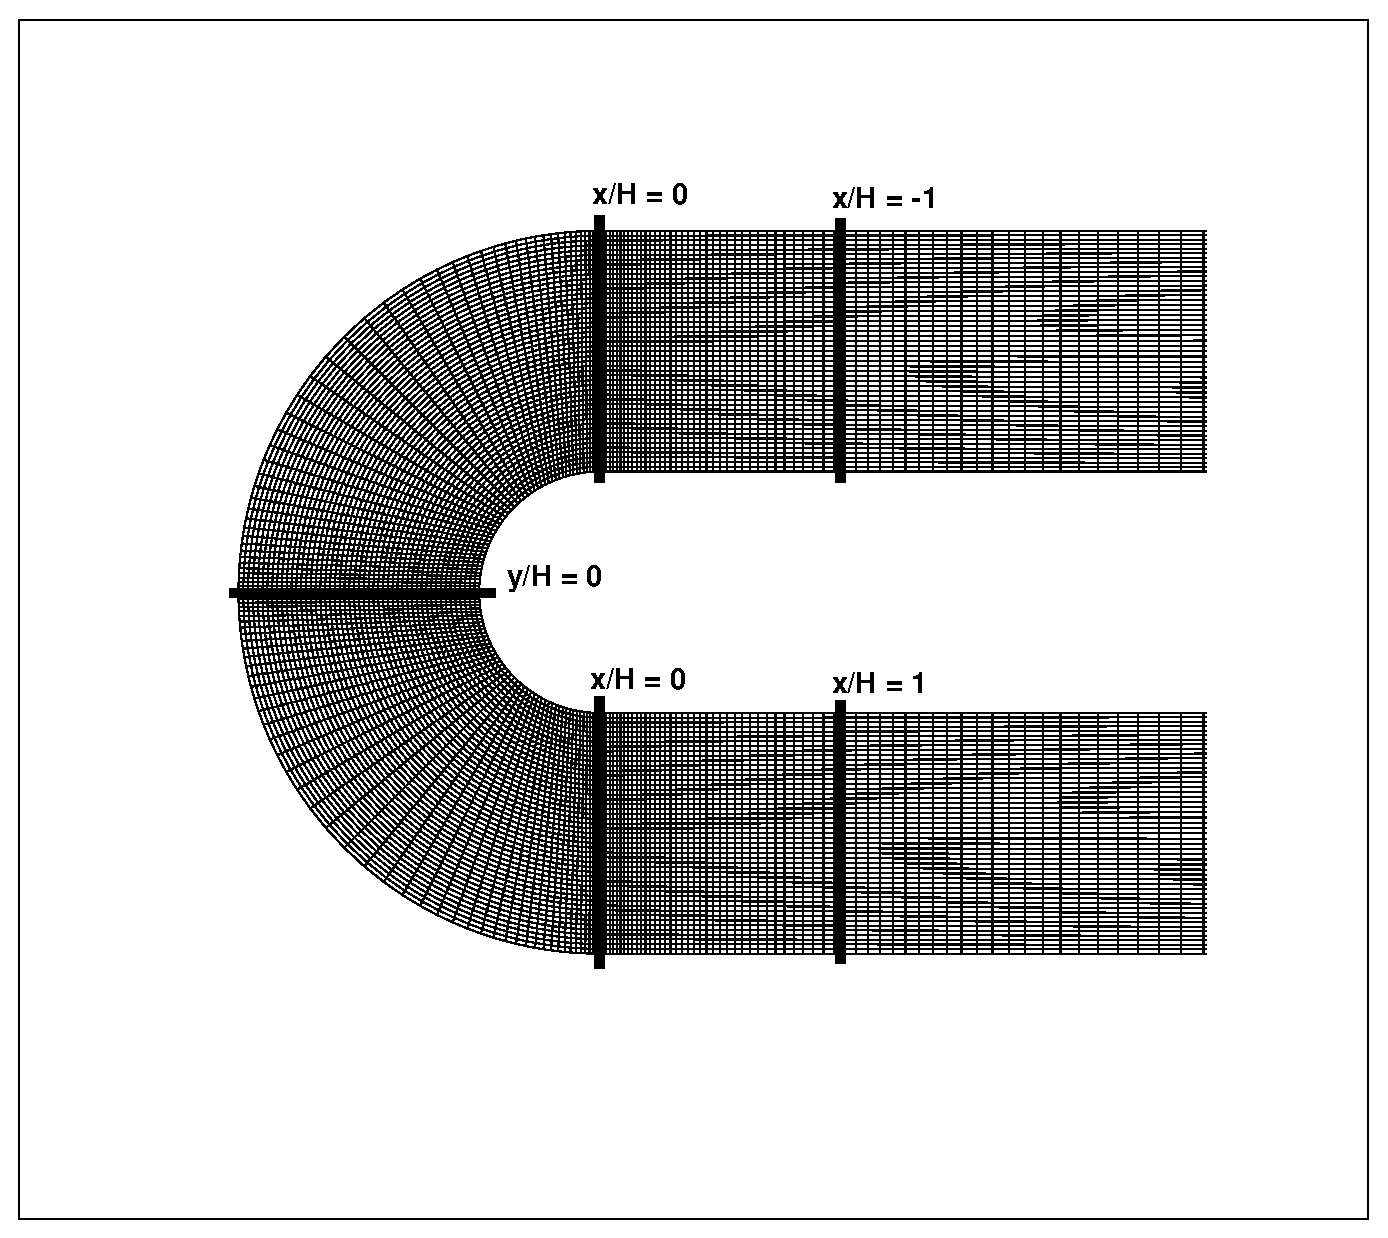
\includegraphics[scale=0.6]{sampleLinesAndMesh}
	\caption{Сетка расчётной области на участке поворота (15000 ячеек)}
	\label{fig:sampleLinesAndMesh}
\end{figure}
На \textit{рисунках \ref{fig:uDuctMeshIndependence1} и \ref{fig:uDuctMeshIndependence2}} показано сравнение решения на сетках 15000 ячеек и 5400 ячеек для поперечной компоненты скорости в сечении $y=0$. Очевидно, решения практически совпадают, что говорит о том, что сетки в 15000 ячеек достаточно для получения адекватного решения. Результаты далее приводятся для этой сетки.
\begin{figure}[ht]
	\begin{minipage}{0.475\linewidth}
		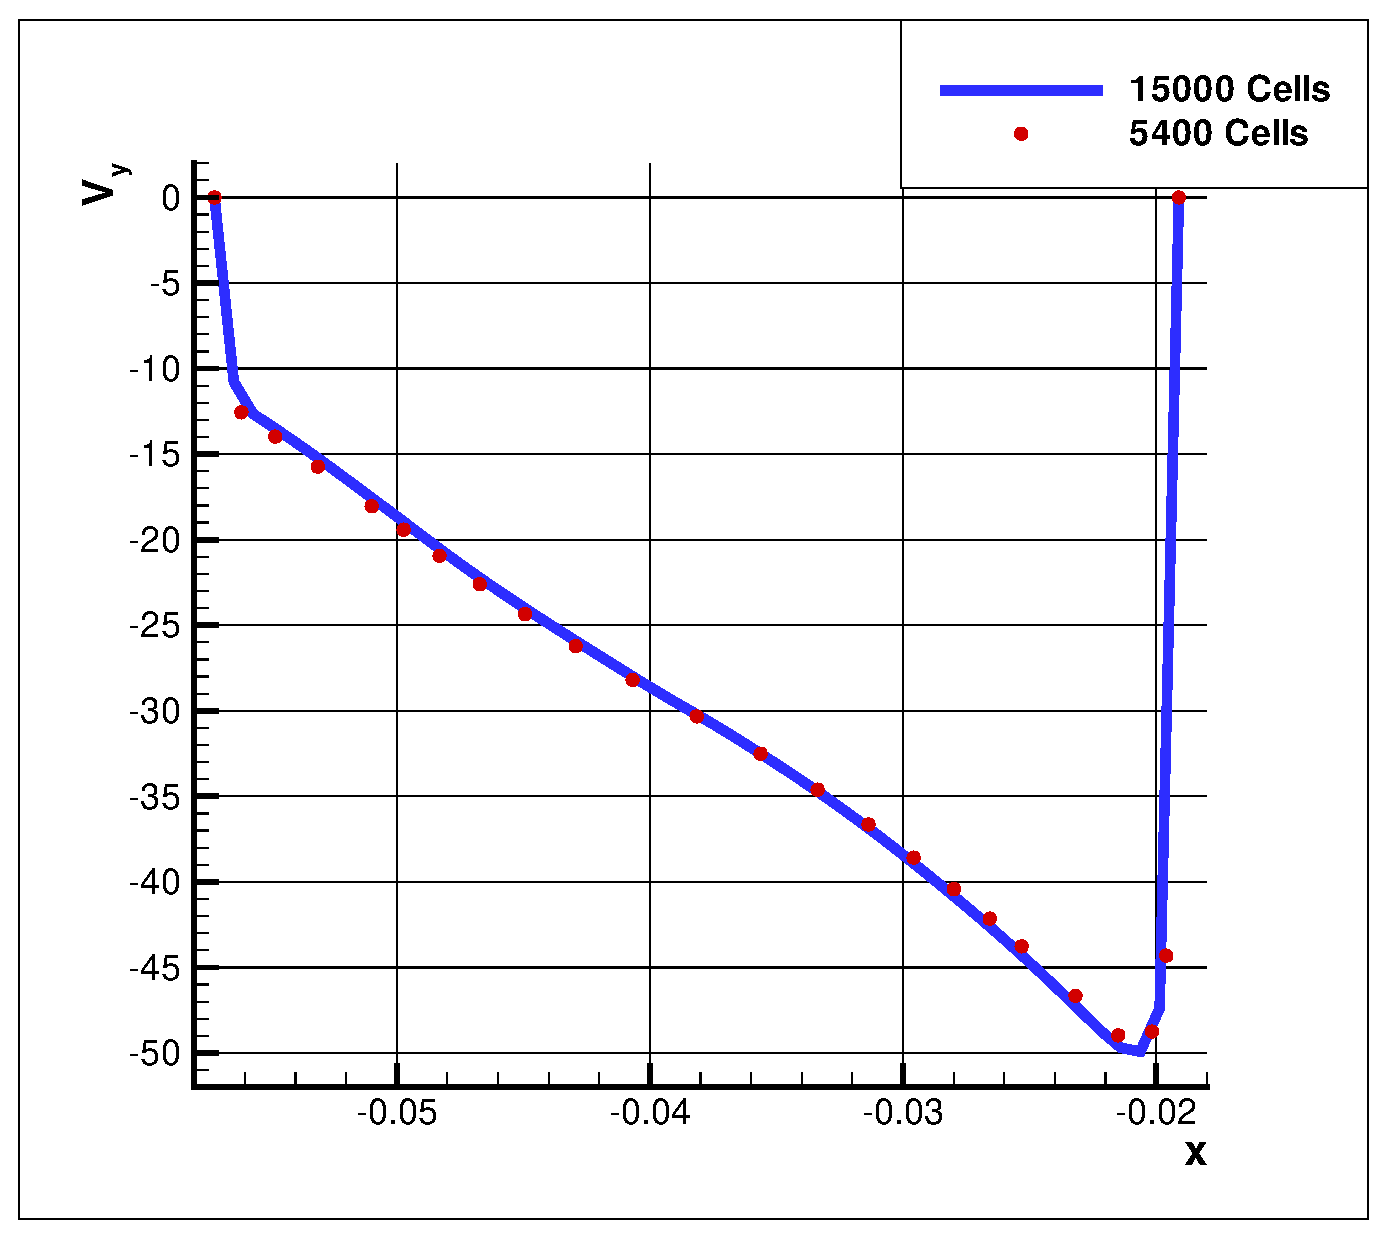
\includegraphics[scale=0.33]{uDuctMeshIndependence1}
		\caption{Сравнение графиков $U_y$ на сетках 5400 ячеек и 15000 ячеек (FLUENT)}
		\label{fig:uDuctMeshIndependence1}
	\end{minipage}
	\hspace{0.5em}
	\begin{minipage}{0.475\linewidth}
		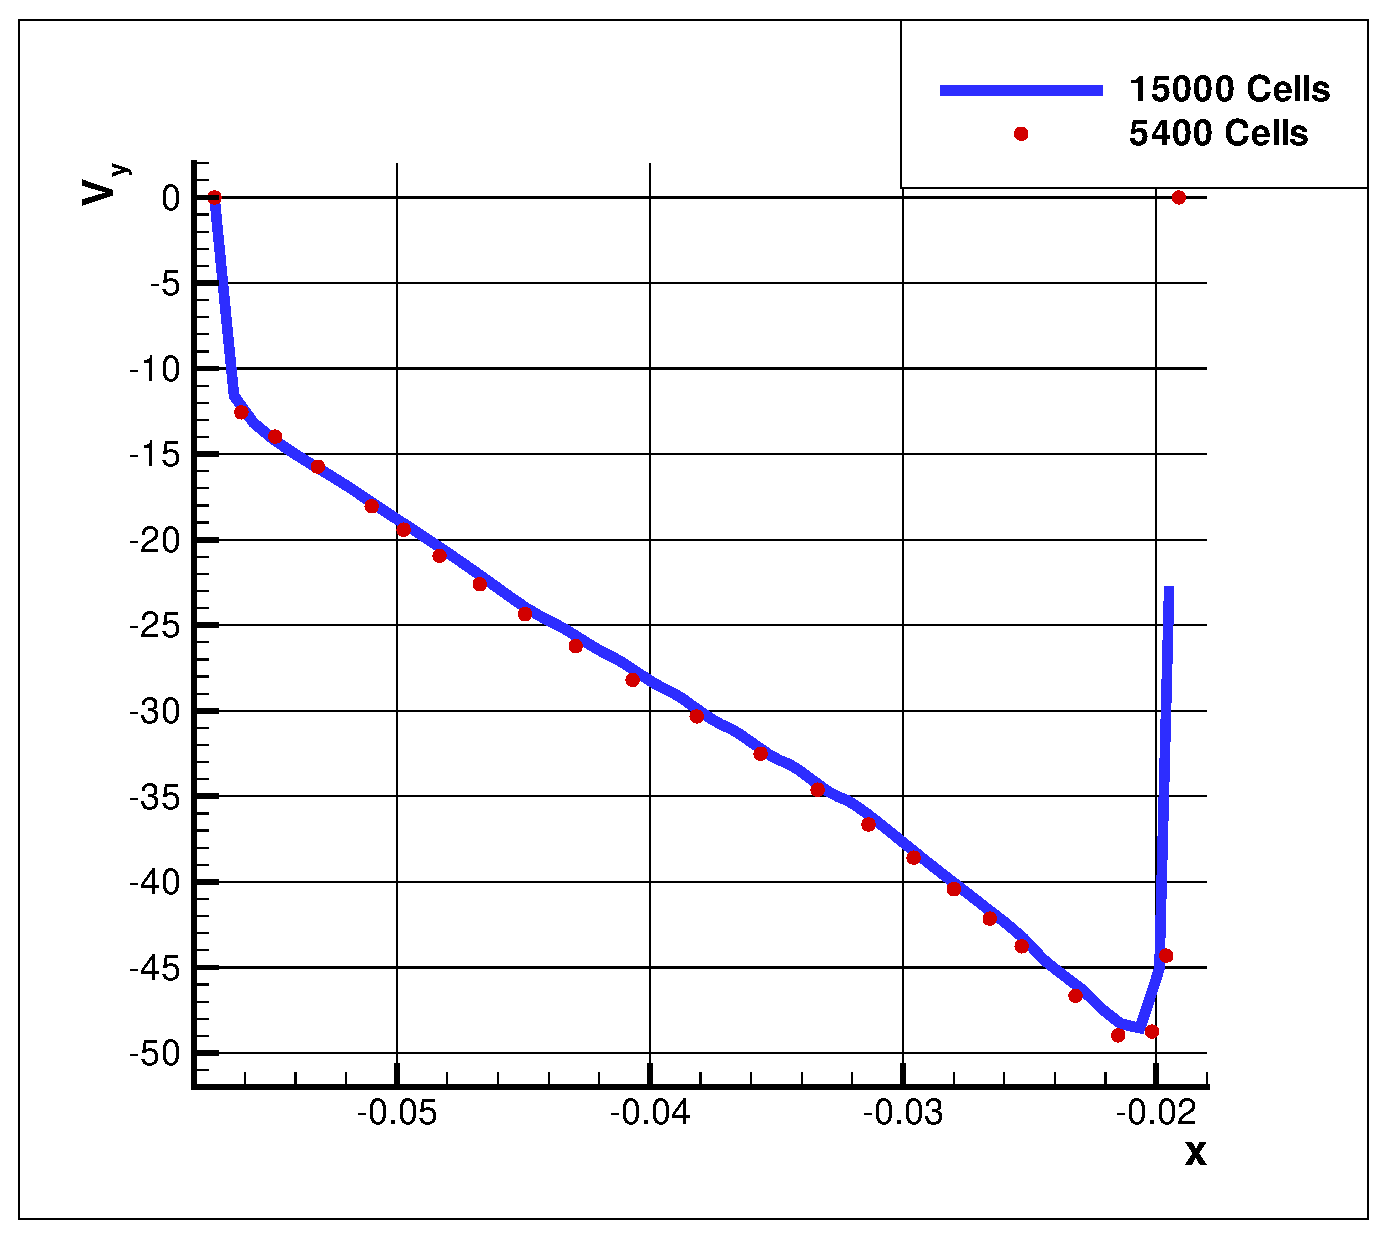
\includegraphics[scale=0.33]{uDuctMeshIndependence2}
		\caption{Сравнение графиков $U_y$ на сетках 5400 ячеек и 15000 ячеек (OpenFOAM)}
		\label{fig:uDuctMeshIndependence2}
	\end{minipage}
\end{figure}
\begin{figure}[h]
	\centering
	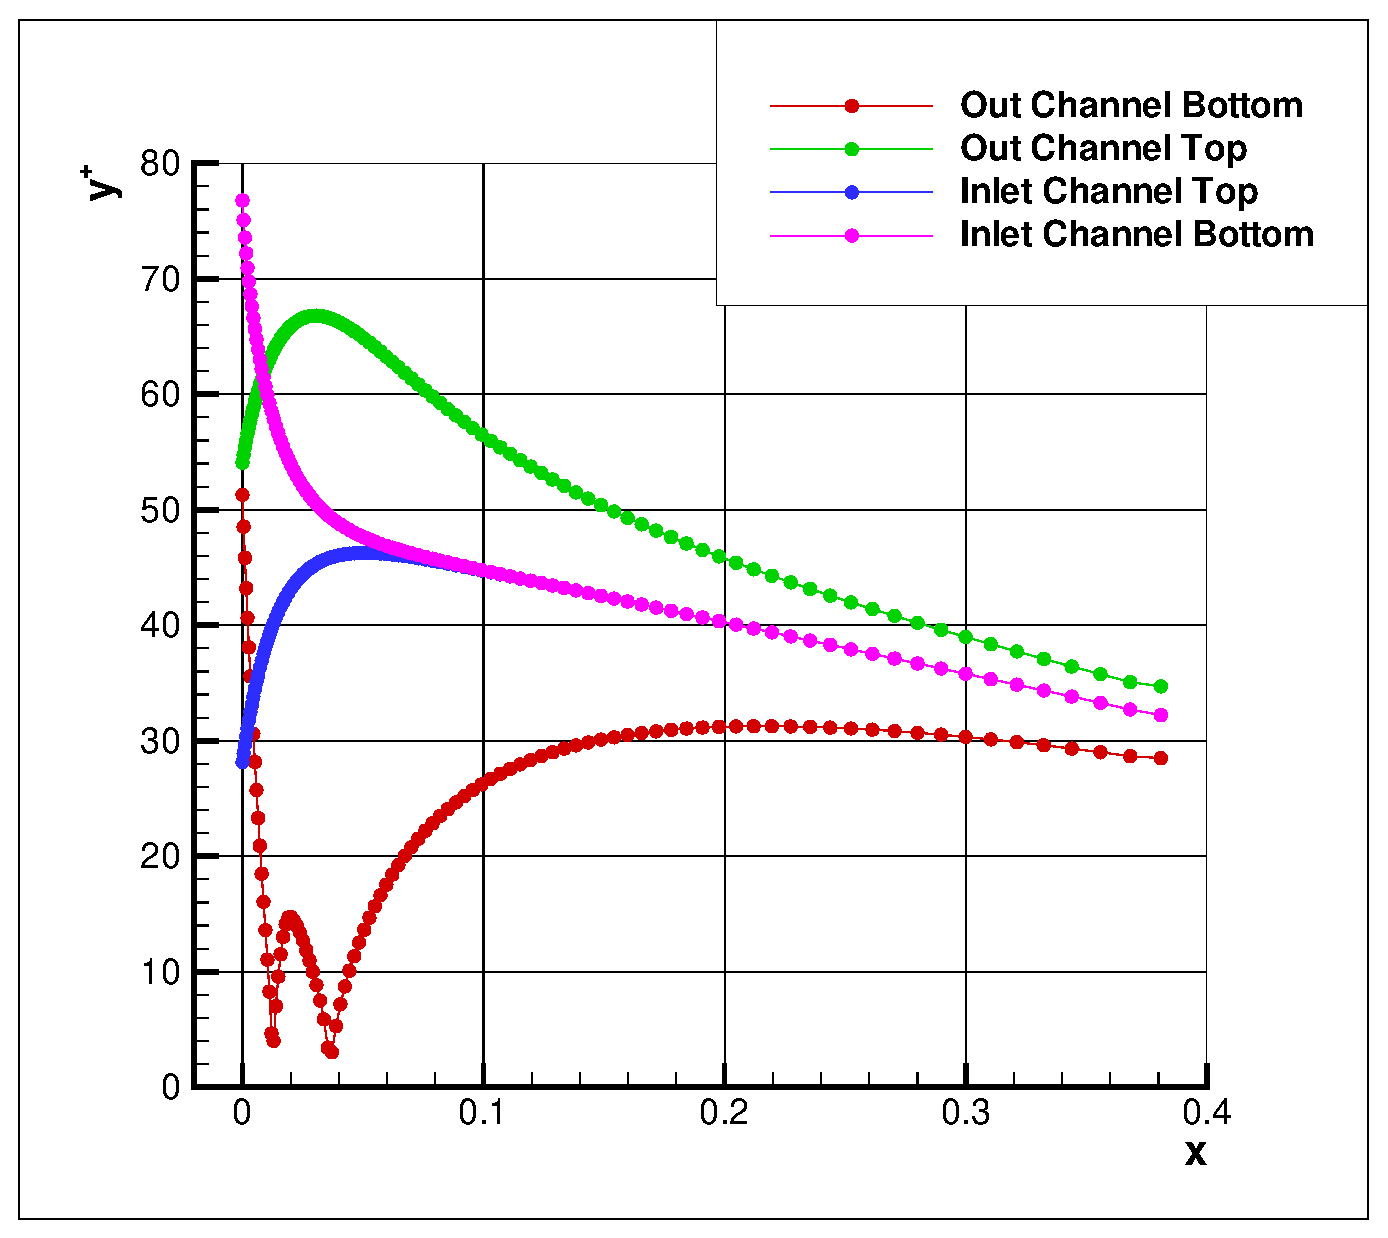
\includegraphics[scale=0.4]{uDuctyplus}
	\caption{Величина $y^{+}$ первой пристенной ячейки на внешней и внутренней стенках}
	\label{fig:uDuctyplus}
\end{figure}
\clearpage

Величина $y^{+}$ \textit{(рис. \ref{fig:uDuctyplus})} для первой пристенной ячейки лежит в пределах $10 \div 80$, что вполне приемлемо для расчётов с использованием автоматических пристеночных функций.

Перейдём теперь непосредственно к сравнению результатов расчёта с экспериментами Монсона и решением в Fluent с использованием встроенной в него поправки к модели Ментера для учёта кривизны линий тока. Для сравнения выбрано 5 поперечных сечений канала \textit{(рисунок \ref{fig:sampleLinesAndMesh})} - $x/H=-1$, $x/H = 1$, $x/H = 0$ (верхний канал), $x/H = 0$ (нижний канал) и $y/H=0$.
\begin{figure}[h]
	\centering
	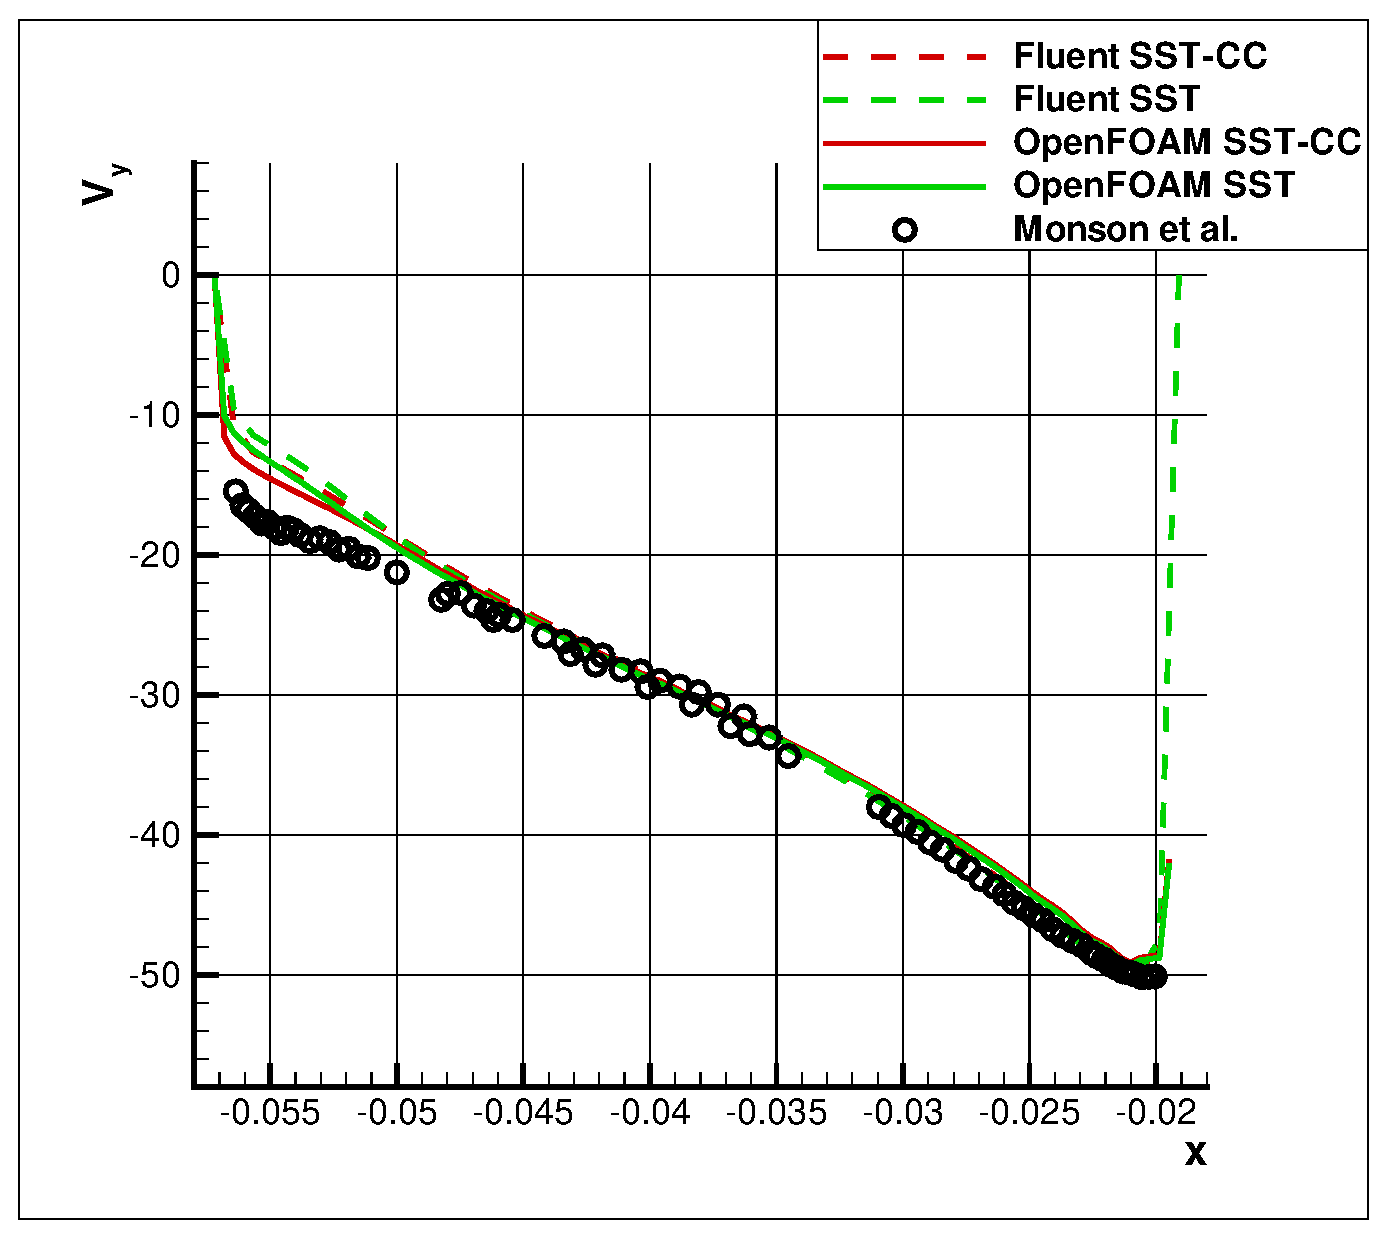
\includegraphics[scale=0.55]{yh0}
	\caption{Профиль поперечной скорости в сечении $y/H=0$}
	\label{fig:y0}
\end{figure}
\begin{figure}[ht]
	\begin{minipage}{0.475\linewidth}
		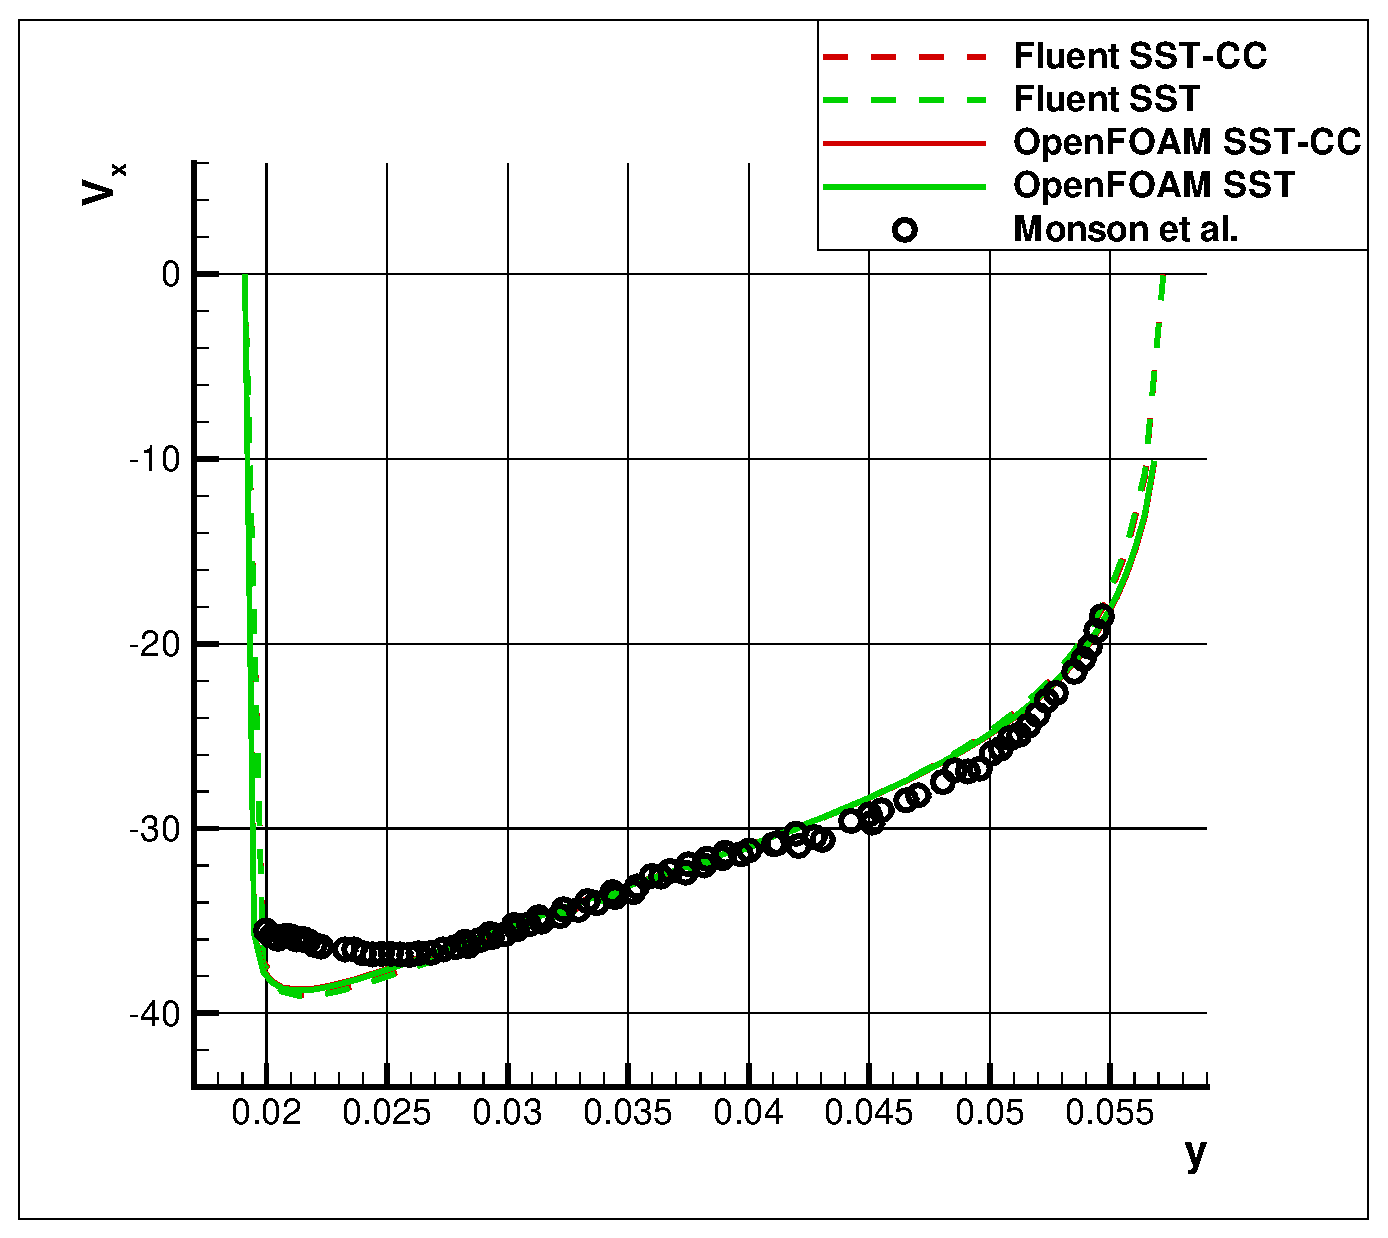
\includegraphics[scale=0.33]{xh0up}
		\caption{Профиль продольной скорости в сечении $x/H=0$ (верхний канал)}
		\label{fig:x0up}
	\end{minipage}
	\hspace{0.5em}
	\begin{minipage}{0.475\linewidth}
		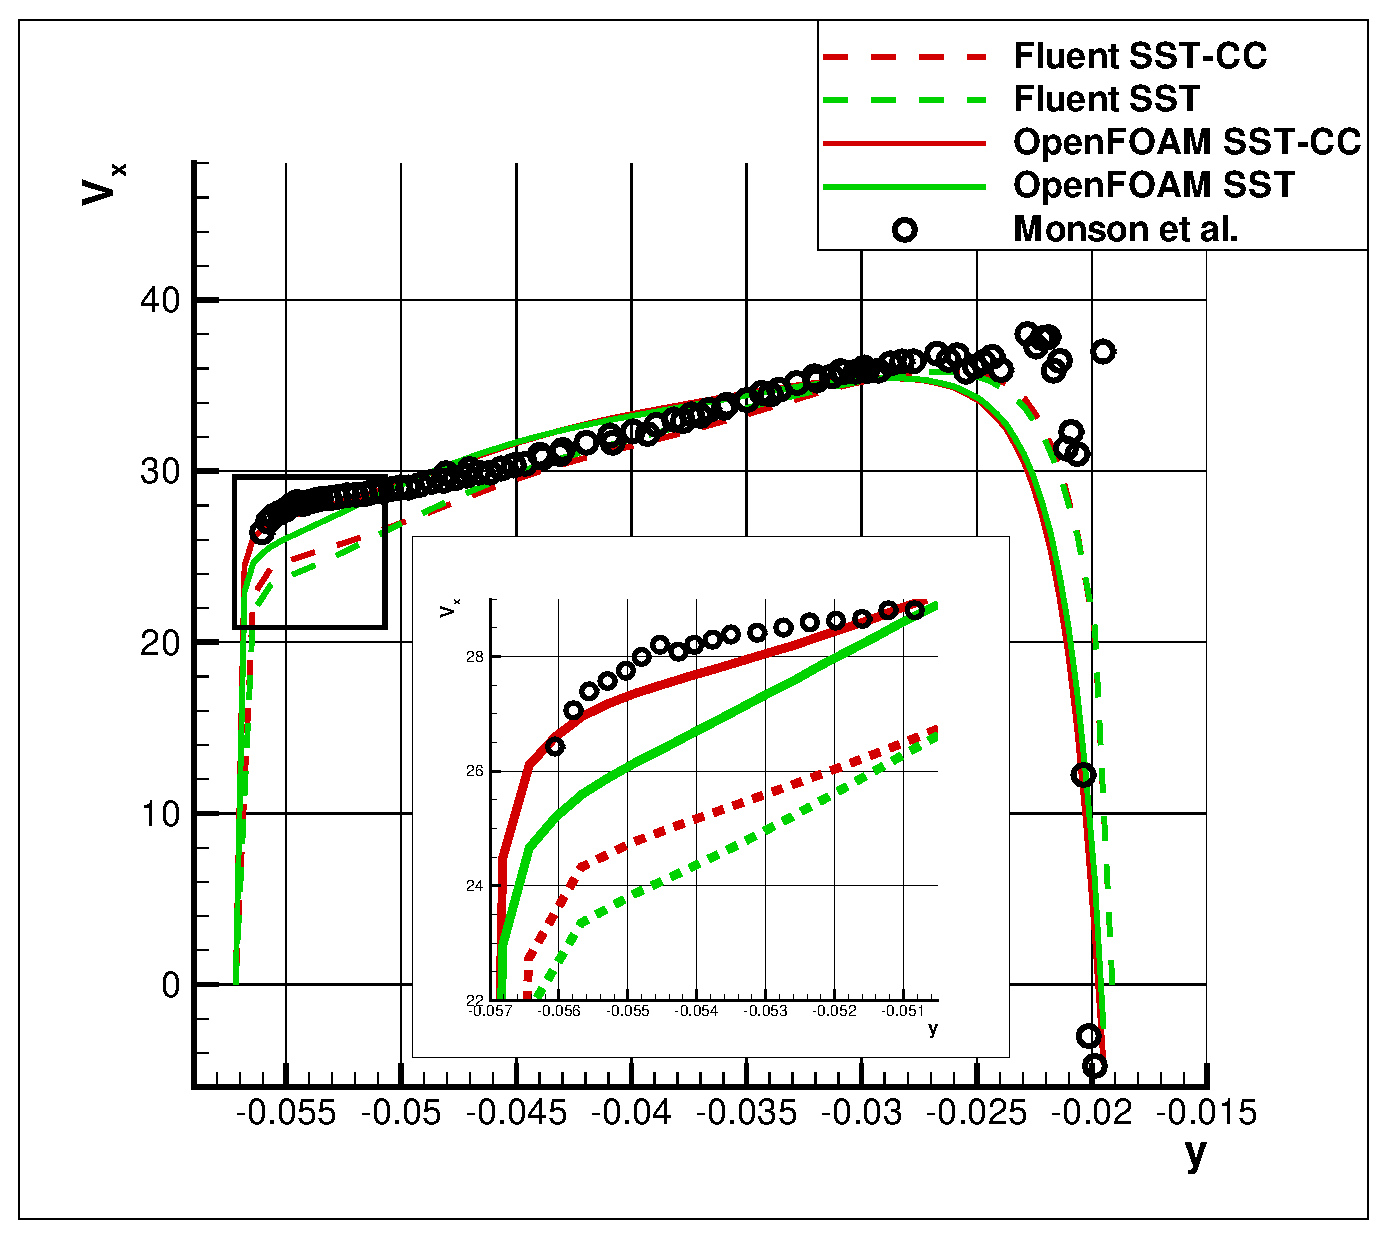
\includegraphics[scale=0.33]{xh0down}
		\caption{Профиль продольной скорости в сечении $x/H=0$ (нижний канал)}
		\label{fig:x0down}
	\end{minipage}
\end{figure}
\begin{figure}[ht]
	\vspace{-1em}
	\begin{minipage}{0.475\linewidth}
		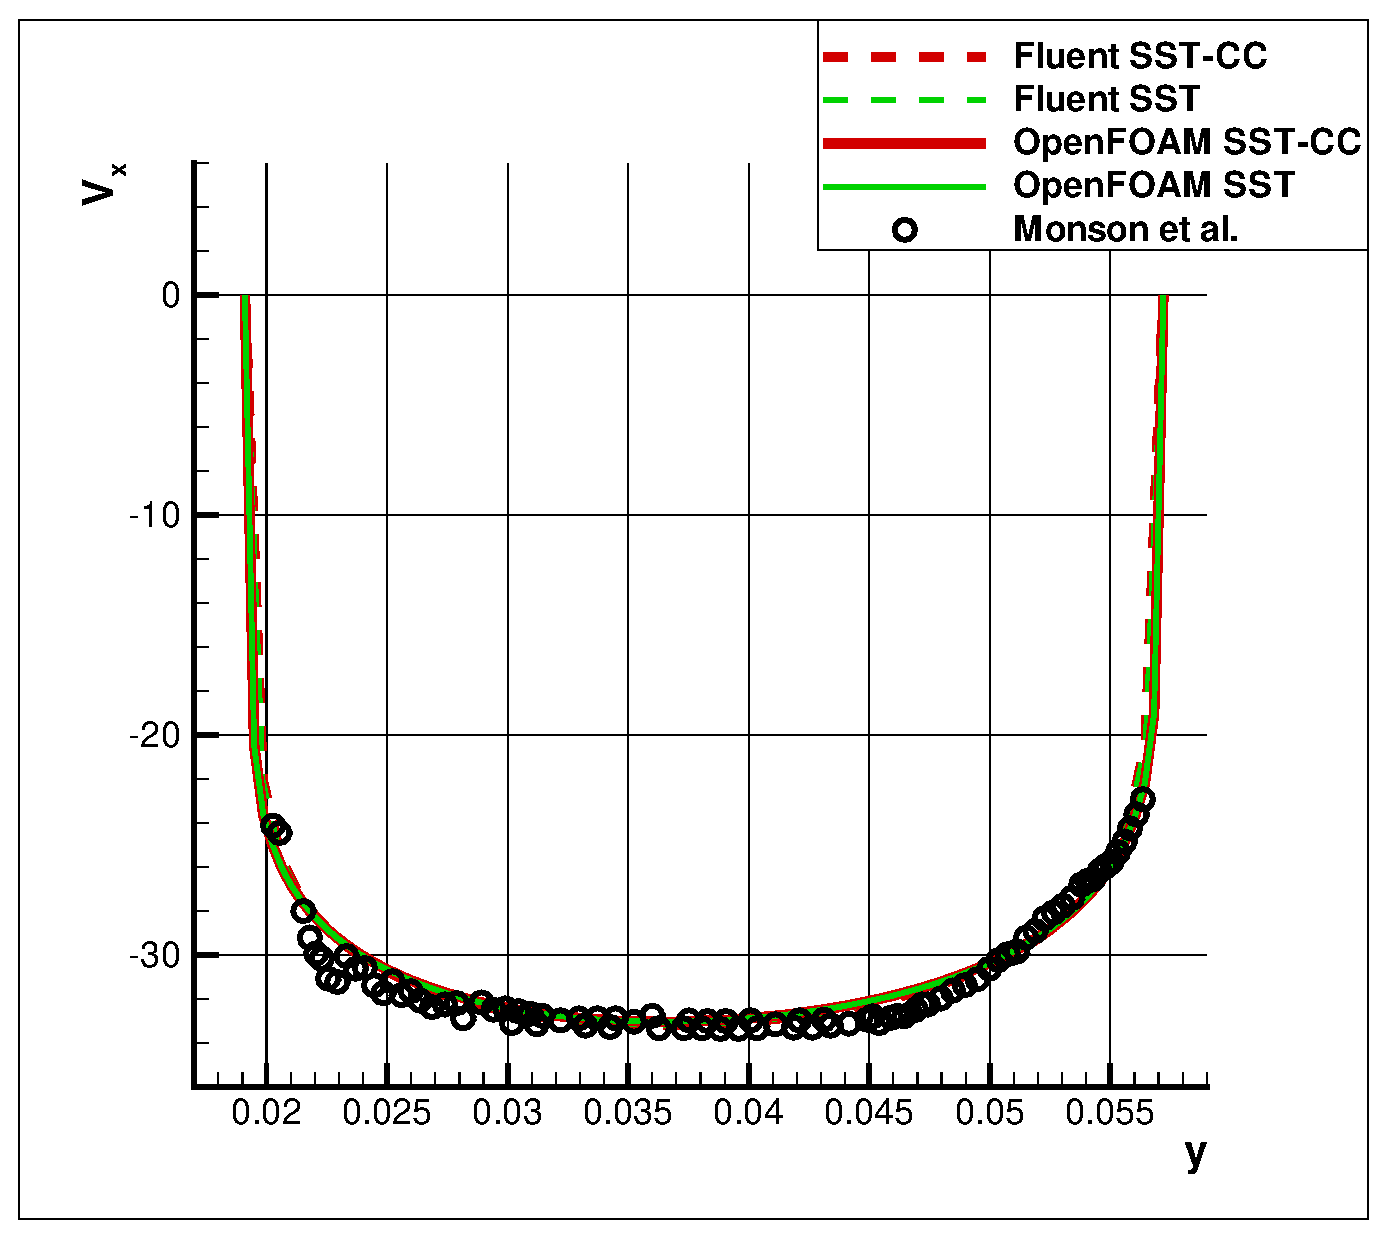
\includegraphics[scale=0.33]{xh1up}
		\caption{Профиль продольной скорости в сечении $x/H=-1$}
		\label{fig:x1up}
	\end{minipage}
	\hspace{0.5em}
	\begin{minipage}{0.475\linewidth}
		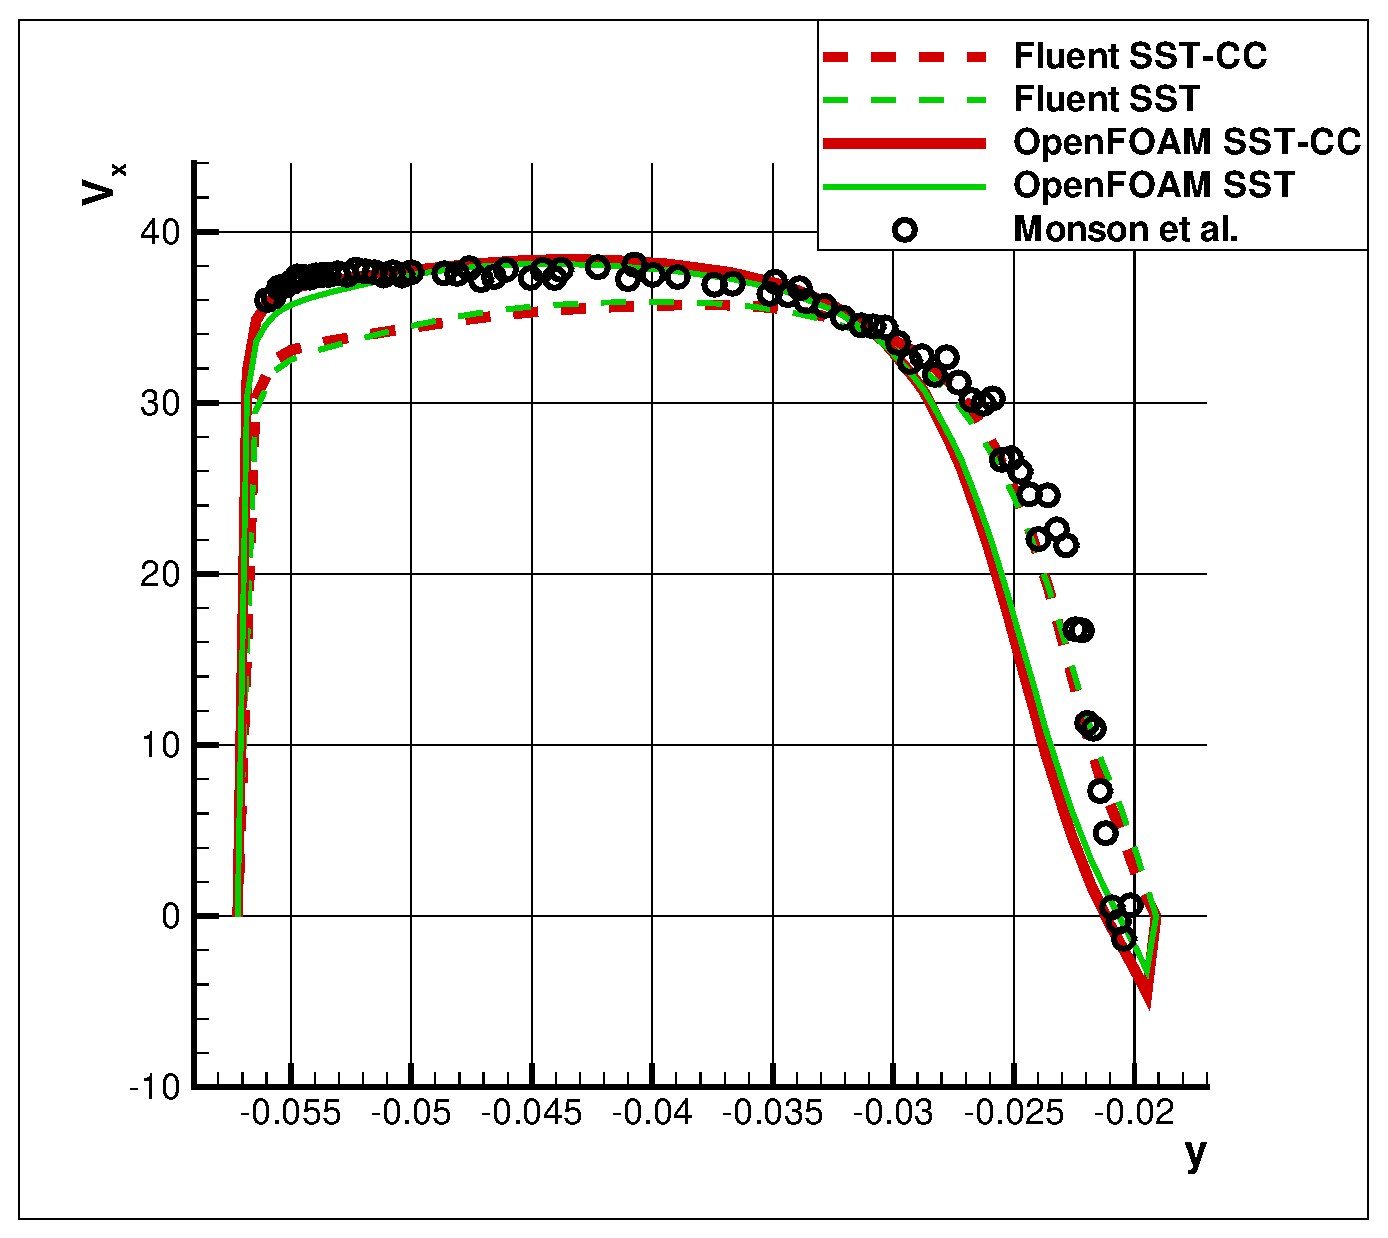
\includegraphics[scale=0.33]{xh1down}
		\caption{Профиль продольной скорости в сечении $x/H=1$}
		\label{fig:x1down}
	\end{minipage}
\end{figure}
\clearpage

Для начала, стоит сказать, что профили продольной скорости на участке перед поворотом \textit{(рисунки \ref{fig:x0up} и \ref{fig:x1up})}, полученные в Fluent и OpenFOAM совпадают с точностью до толщины линии и очень хорошо соответствуют экспериментальному течению. Это говорит о том, что базовая модель Ментера, выбранная для введения поправки, правильно предсказывает течение на прямолинейном участке канала.

Из \textit{рисунков \ref{fig:y0}, \ref{fig:x0down} и \ref{fig:x1down}} видно, что профили скорости, полученные с использованием модифицированной модели Ментера гораздо ближе к экспериментальным данным в пристеночной области криволинейной части канала, чем решение, полученное с использованием стандартной модели. Поправка, при этом, как и следовало ожидать, не влияет на прямолинейное течение в зоне перед поворотом \textit{(рисунки \ref{fig:x0up}, \ref{fig:x1up})}.

Влияние поправки сильнее всего заметно на выпуклой внутренней стенке, генерация турбулентности на которой в немодифицированной модели Ментера занижена. Надо заметить, что результаты, полученные с использованием OpenFOAM при этом лучше согласуются с экспериментами Монсона, чем результаты расчётов в Fluent. Это, однако же, несправедливо для вогнутой внешней стенки. Здесь результаты расчётов в Fluent, наоборот, ближе к экспериментальному профилю. Видно также, что на вогнутой стенке ни в Fluent, ни в OpenFOAM поправка практически не влияет на течение.

В целом, очевидно достаточно сильное положительное влияние введённой поправки, учитывающей кривизну линий тока, на результаты расчётов.